\section{Data Wrangling and Data Cleaning}
\label{subsec:dataCl}


The data cleaning process was done in two steps:

\begin{itemize}
\item For yellow and green cap trips, the rows that have distances equal to $0$ we deleted. This, because we are aiming to take into account only the trips that traveled some distance.
\item For yellow and green caps trips, the IQR methodology was used to clean the outliers from the data. A variable called ``amount\_per\_distance'' was created. It was calculated as the ratio between ``total\_amount" and ``trip\_distance". With this new variable, the values that did not show a common relationship between distance and values were deleted.
\end{itemize}

Feature engineering:
We created a new variable that measures the ratio between the total amount of the trip and the distance it traveled. This feature was created for Yellow trips and Green trips and was used for the outlier cleansing.

\subsection{Data Analysis}

Different plots were created with the aim to understand the behaviour of the different transportation systems. The following plots summarize the important findings encountered, so far.

Figure \ref{fig:boxTrips} shows the graph plots of the monthly trips for the different transportation systems: Figure \ref{fig:a} for Uber's trips, Figure \ref{fig:b} for Yellow cap trips, Figure \ref{fig:c} for Green cap trips, and Figure \ref{fig:d} for MTA trips. The boxplots differentiate the trips between rush hours (orange boxes) and non-rush hours (blue boxes). From the figure it can be seen that the MTA is highly used in rush hours. Additionally, it is possible to see that there has been a significan increase of the number of trips taken by Uber from 2015 both in rush and non-rush hours; and a decrease on the number of trips taken by Yellow caps, especially in rush hours. 

\begin{figure}%
\centering
\subfigure[Uber trips.]{%
\label{fig:a}%
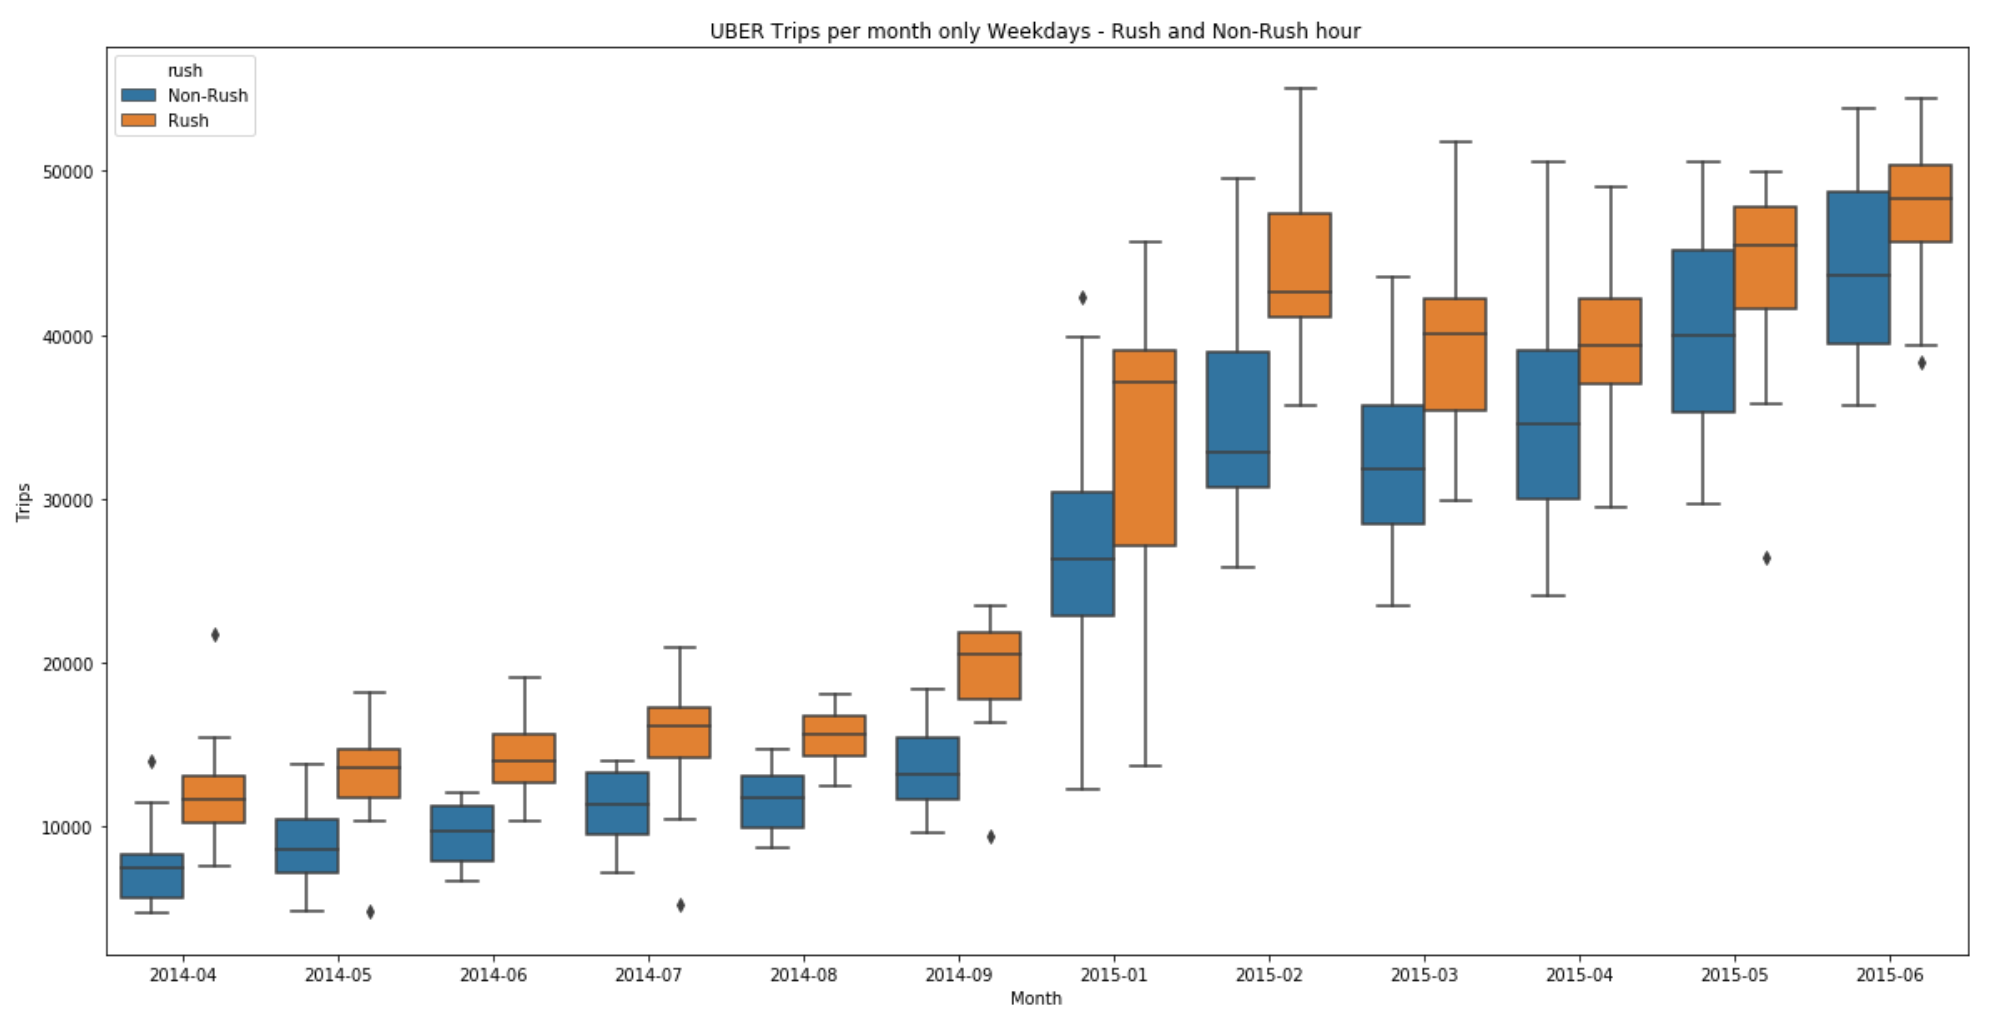
\includegraphics[height=2in, width=3.5in]{UBER_trips_only_weekdays_rush_and_non_rush.png}}%
\qquad
\subfigure[Yellow cap trips]{%
\label{fig:b}%
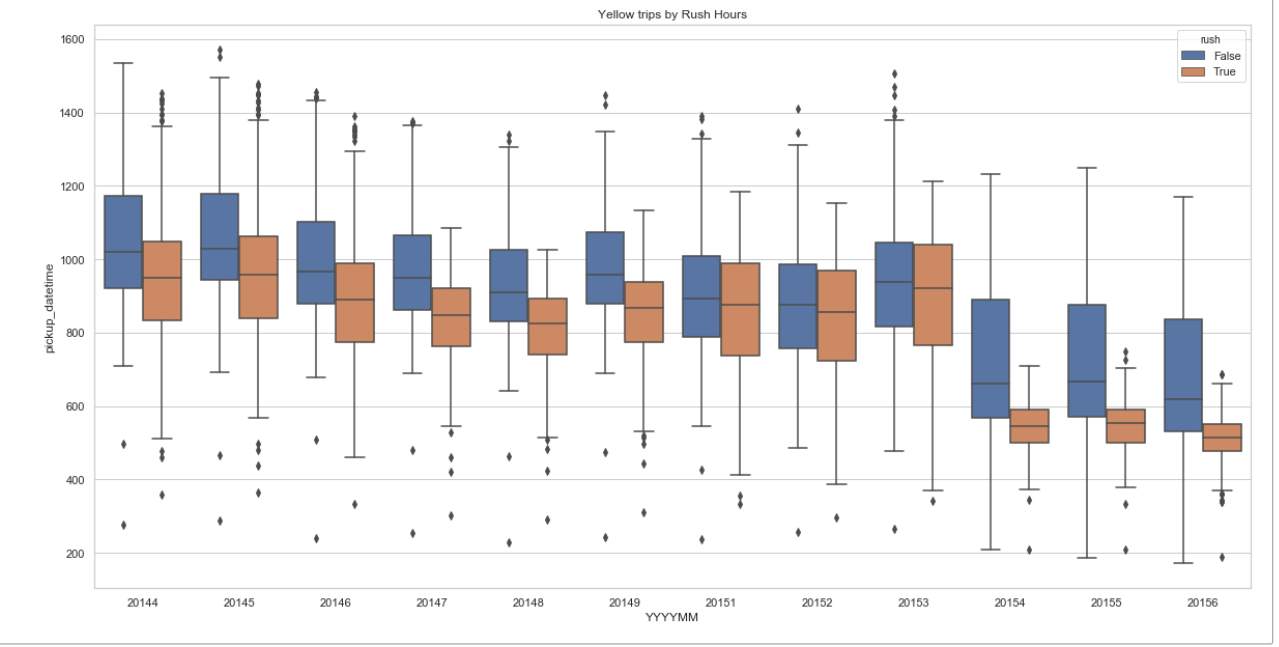
\includegraphics[height=2in, width=3.5in]{yellowTripsRushHours.png}}%
\qquad
\subfigure[Green cap trips]{%
\label{fig:c}%
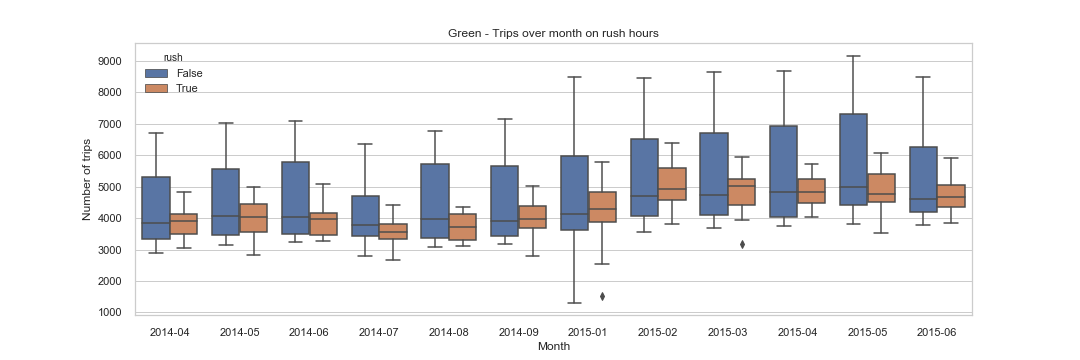
\includegraphics[height=2.4in, width=3.5in]{green_trips_month_rush.png}}%
\qquad
\subfigure[MTA trips]{%
\label{fig:d}%
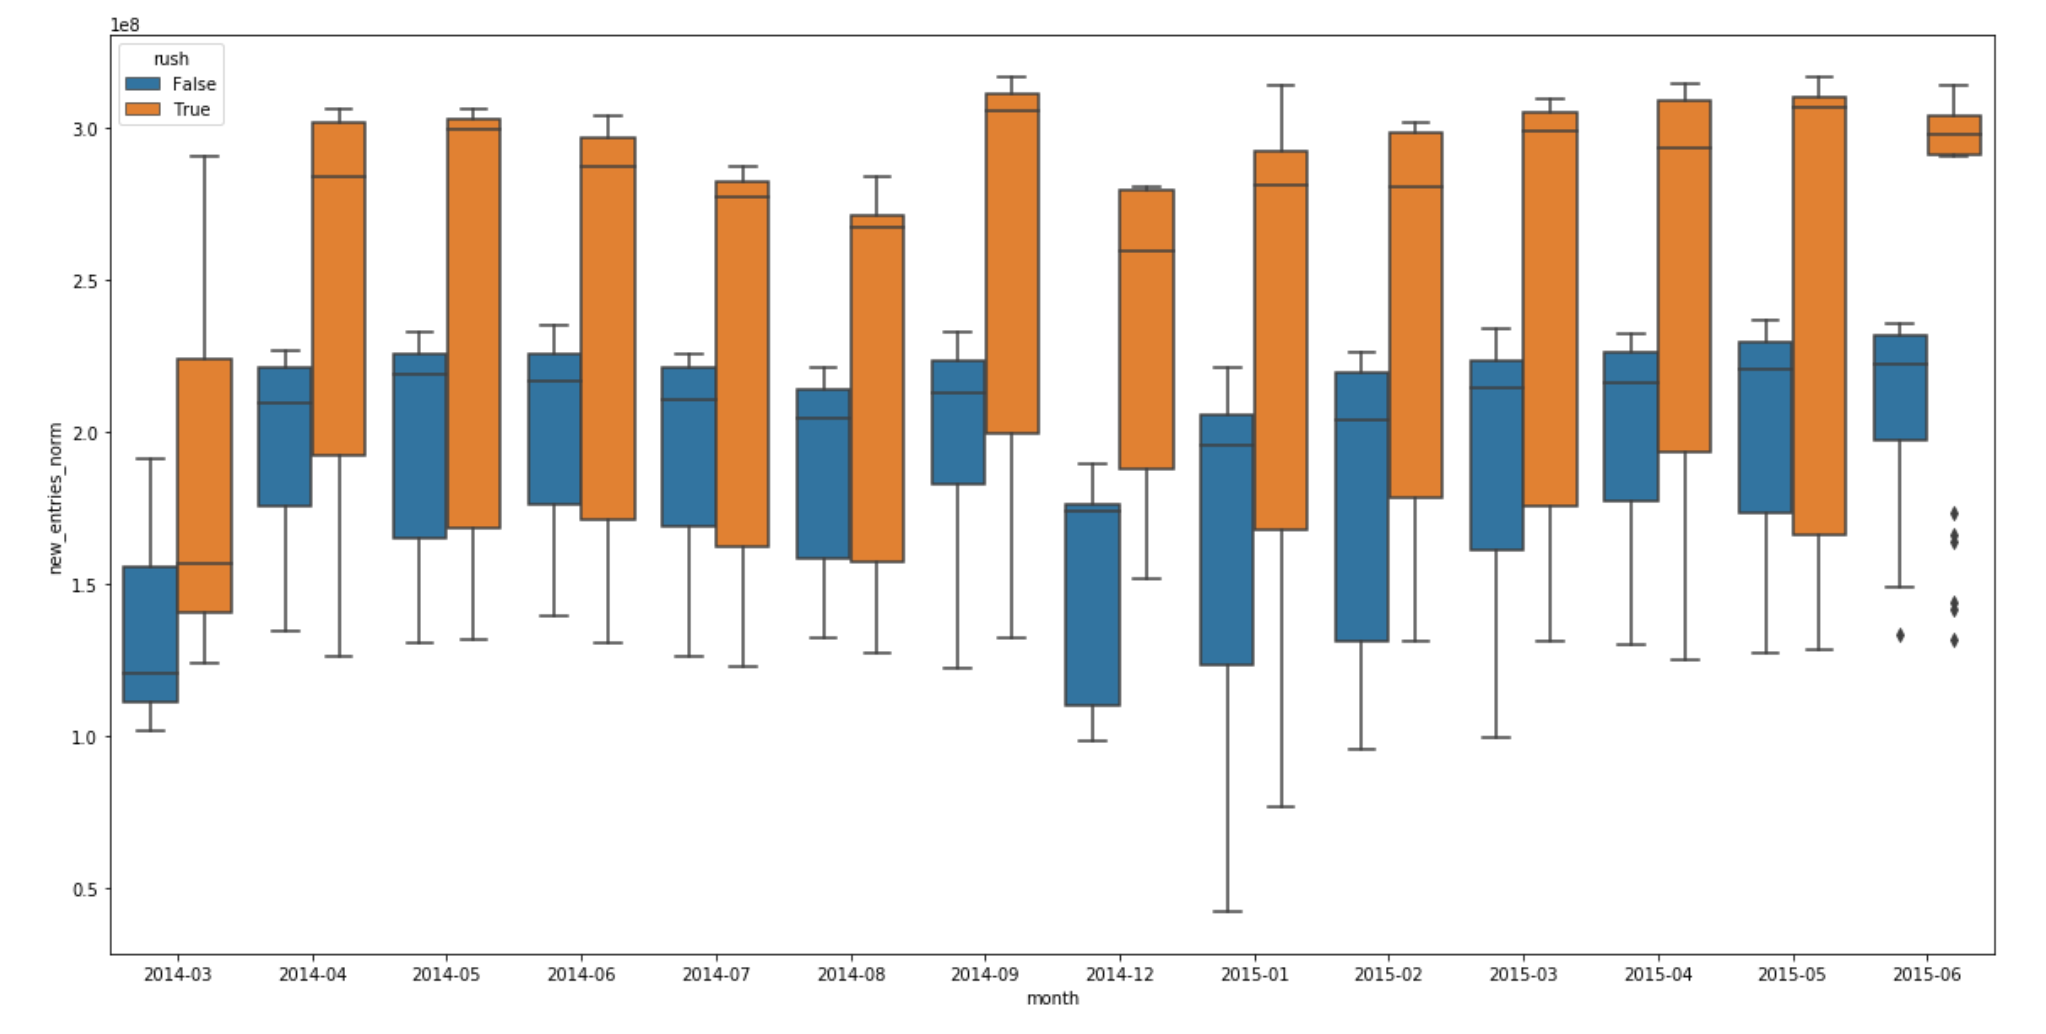
\includegraphics[height=2in, width=3.5in]{mta_new_entries_orange_rush_hour.png}}%
\caption{Monthly behaviour of the number of trips. Orange boxes represent the number of trips in rush hours and blue ones correspond to non-rush hours. }
\label{fig:boxTrips}%
\end{figure}



Figure \ref{fig:boxDistances} compares the monthly average travel distance covered by Uber and Yellow caps. From these plots, it is possible to see that from 2015, Uber is widely used for long distance trips, in contrast to Yellow caps. On the other hand, the average travel distance of Yellow caps experienced an increase in April 2015. 


\begin{figure}%
\centering
\subfigure[Uber]{%
\label{fig:first}%
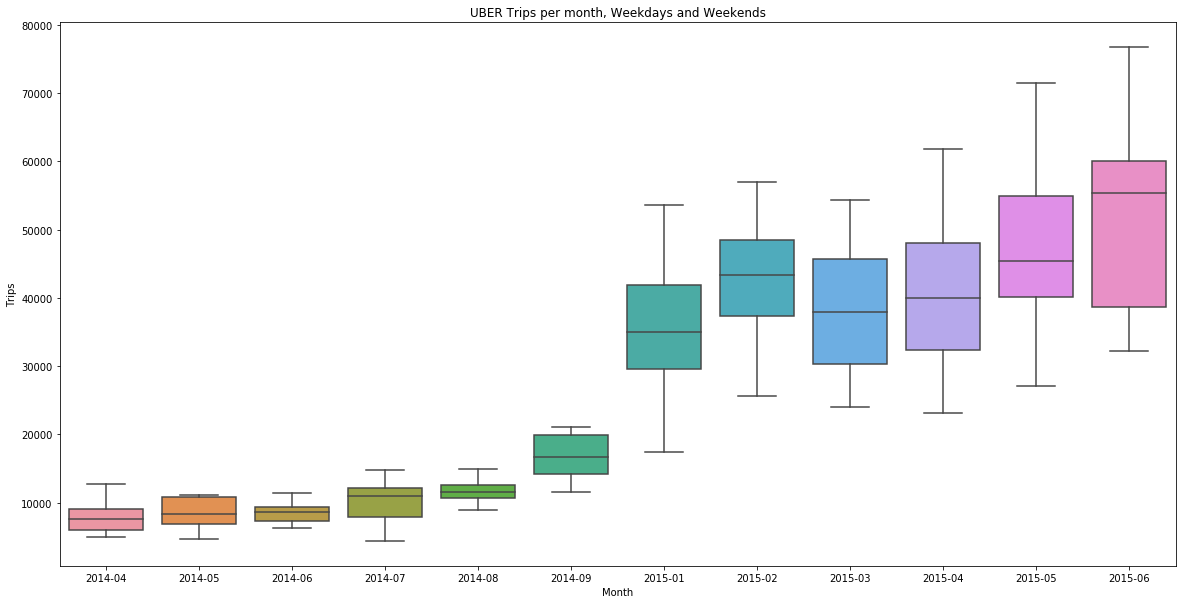
\includegraphics[height=2in, width=5in]{UBER_Trips_per_month_only_weekends.png}}%
\qquad
\subfigure[Yellow caps]{%
\label{fig:second}%
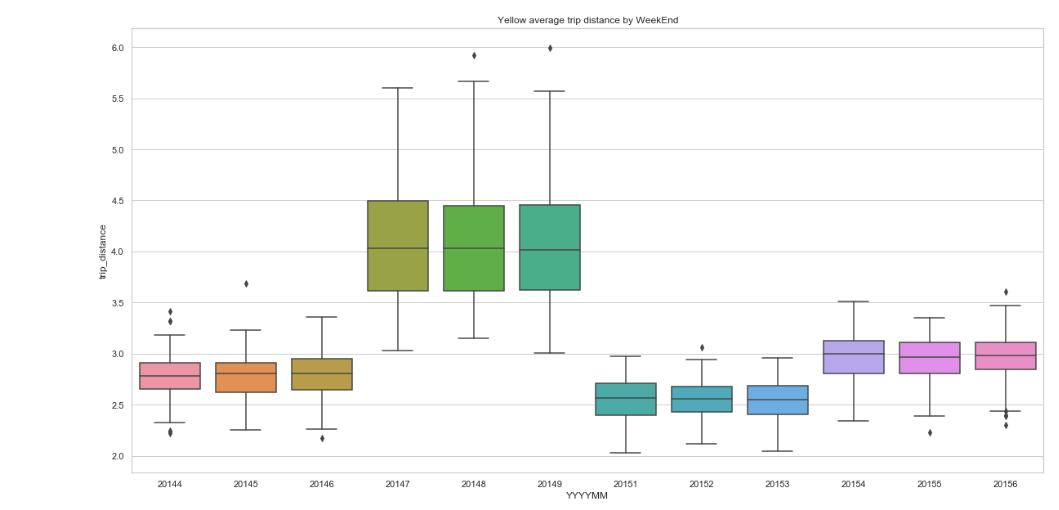
\includegraphics[height=2.2in, width=5.5in]{Yellow_Cabs_Average_trip_distance_Weekend_Only_by_Month_copy.png}}%
\caption{Comparison of the monthly average travel distance covered by Uber and Yellow caps. From the plot  }
\label{fig:boxDistances}%
\end{figure}
